\documentclass[../main.tex]{subfiles}

\begin{document}

\chapter{Việt Phương - Người lữ hành cô đơn}

\begin{subtitle}

(Về tập thơ Cửa đã mở, NXB Thanh Niên, 2008)

\end{subtitle}

\begin{metadata}

\begin{flushright}21.3.2008\end{flushright}

Hoàng Vũ Thuật

Nguồn: Báo Văn Nghệ số 11, 15.3.2008

\end{metadata}

\begin{multicols}{2}

\begin{figure}
	\centering
	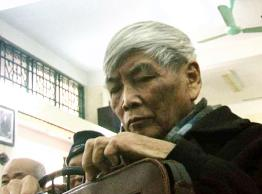
\includegraphics[width=\textwidth]{../img/tho210308.jpg}
	\caption{Nhà thơ Việt Phương}
\end{figure}
 Nhà hoạt động xã hội, xét mặt nào đó, gương mặt họ khó nhận diện một cách đầy đủ. Vào thời điểm lịch sử nhất định, họ hiện ra đúng họ, rồi có thể mất đi hoặc tồn tại cùng thời gian. Còn một học giả, một trí thức, gương mặt dễ nhận biết, vì họ mang trong mình những dự cảm xã hội và khát vọng muôn thuở của con người. 
 
Hình ảnh con người từ lâu đã là tâm điểm sáng tạo của thơ Việt Phương. Ông luôn đề cao con người, một chữ người viết hoa, dù dưới góc nhìn nào, thời điểm nào. Ở tập thơ \textit{Cửa mở} do nhà xuất bản Văn Học ấn hành năm 1970, có một chú thích trong bài thơ "Ta nhìn trời đêm nay và ta đọc", được ghi: \textit{Chữ người bị phá tung ra và chắp lại thành NƠI GỪI, }đủ hiểu ông quan tâm và nhận thấy thân phận con người đang bị dày vò, đạo lí con người đang bị chà đạp tới lúc cần báo động. Con người trong thơ Việt Phương mang tính nhân loại, thoát khỏi mọi ranh giới vốn được qui rập công thức, duy lí. Nhưng hình ảnh  lại rất cụ thể, gần gũi, rất cội rễ, không chút ảo hoá, huyễn tưởng: 
\begin{blockquote}
        
\textit{Anh chưa đến hai mươi mà thấy mình già lắm}        
\textit{Sống thường trực của anh là lợm giọng}        
\textit{Chán chường muốn mửa cuộc đời ra}        
\textit{Mửa cả tiếng chim mửa cả màu hoa}        
\textit{Anh nhìn đâu cũng thấy điều đã quá nhiều lần nhìn thấy}        
\textit{Cả những con người cũng lặp đi lặp lại thành thiu chảy}        
\textit{…}        
\textit{Anh tự biết mình là tinh chất của rỗng không} 
\textit{Mà gân anh săn mà máu anh hồng} 

\end{blockquote}
 
Khát vọng cao cả giải phóng con người thường trực xâu chuỗi thành chất triết luận trong thơ Việt Phương. 
 
\textit{Cửa đã mở}  tiếp tục dòng chảy ấy. Qua thăng trầm trải nghiệm, mạch suy tưởng triết luận càng sâu đậm, nhân tình hơn. Ông luôn dành cho độc giả những điều mới mẻ và khác lạ. Không là kiểu khác lạ của lối thơ khước từ nghĩa, khước từ sự hiểu, mà sự khác lạ bắt nguồn từ một nhân sinh quan, thế giới quan, một thông điệp: \textit{Sự chưa biết của con người là vô cùng vô hạn / Biển mênh mông người mới chỉ quẩn quanh bên mạn con tàu / Cái gì con người làm ra cũng chưa đâu vào đâu và nông cạn / Chỉ tác phẩm của thánh thần hay ma quỉ là tuyệt vời bài bản trước sau }(“Ngỏ”). Ông nhìn thẳng vào sự thật như nhìn vào đường vân để biết giá trị đời sống: \textit{Sự sống cố tình xấu xí từng đường vân }(“Gần”). Một nhận định, một sự bừng thức, một tâm trạng? Hiểu sao cũng được, mỗi khi trái tim nhà thơ rung động cùng thân phận con người. 
 
Không gian vô biên của vũ trụ, nhờ ánh sáng chiếu soi mà nhìn thấy được. Nhưng nếu không có con người thì vũ trụ cũng chỉ là bóng tối, một khối lặng câm. Nhờ nhận thức con người mà thấu hiểu qui luật của vũ trụ, thấy được chuyển hoá của thiên nhiên: 
\begin{blockquote}
 
\textit{Có vũ trụ nằm im bặt dưới hàng mi ta} 
\textit{     }
\end{blockquote}

\textit{      } 
 Và: 
   \begin{blockquote}
                                
\textit{Có một mùa xuân để chùi như chiếc mùi soa}        
(“Có”) 
  \end{blockquote}
           
Minh triết lắm mà lãng mạn lắm. Vị thế hai câu thơ trên thuộc về con người. Chỉ có \textit{trí óc và trái tim người} mới thiết lập được mối quan hệ rộng lớn. Người xưa nói: \textit{Người tai mắt đứng trong thiên địa} là vậy. 
 
Thời điểm nào Việt Phương cũng có con mắt biện chứng, không xu thời hệ luỵ: \textit{Bao nhiêu đêm loang lổ / Những vì sao ánh mắt những vì sao bãi đờm }(“Xa”)\textit{, tất cả có cái gì giả nồng nặc giả tanh tưởi giả như một bộ phim con lợn quá dài như một trò đùa dai vô duyên }(“Nhìn”), \textit{Những học thuyết phòi ra như nấm dại }(“Bến”)\textit{, Có lúc trời xanh như tội ác đang đùa }(“Về”)\textit{, Thừa sách thừa bài thừa lí luận / Nửa phần ma quỉ nửa thần tiên} (“Có”). 
              
Nhân loại hàng nghìn năm qua đã phải sống trong những thảm kịch, con người phải gánh trên lưng mình những nghịch lí. Con người bị huyễn hoặc, hoặc tự huyễn hoặc chính mình. Văn học luôn tìm cách cảnh báo, giúp con người nhận thức và tìm cách thoát khỏi những điều trái ngược phi lí ấy. Vì thế nhà thơ là \textit{người lữ hành cô đơn}, một mình xuyên qua bão cát cuộc đời để tìm ra chân lí của lẽ sống, tìm tới cái ý nghĩa nhân văn của cuộc sống. Cô đơn trong thơ ông đâu phải là cô đơn của một kẻ lẻ loi buồn chán, mà là sự cô đơn của một con đường thơ, của một bản ngã, là đường biên thẩm mĩ để làm nên sự sáng tạo độc đáo: 
\begin{blockquote}
        
\textit{Anh thèm khóc thèm cười thèm nổ tung tan tác}        
\textit{Người bộ hành cô đơn trong bão cát mịt mù}        
\textit{Con khủng long vẩn vơ nghe thủy triều dào dạt} 
\textit{Trời biển hoàng hôn rờn rợn hoang vu} 
        
\textit{Anh thèm thực thèm hư thèm cháy bùng rừng rực}        
\textit{Vú em tròn trên khuôn ngực mảnh mai}        
\textit{Trăng mang mang suốt đêm dài trằn trọc}        
\textit{Sao không tên soi trái đất không người}        
(“Lá”) 
     \end{blockquote}
          
Có lẽ đồng cảm với con người và thơ qua tập \textit{Cửa mở }, một sự kiện văn học đầu thập niên 70, mà đại tướng Võ Nguyên Giáp đã làm mấy vần thơ buông tặng Việt Phương lúc ông đã vào tuổi 60. Sự gặp gỡ duyên kì ngộ của hai tâm hồn văn hoá bộc bạch trong âm điệu ý nhị: \textit{Ê a, ê a / Trẻ mãi, ê a, trẻ mãi không già… a a / Trong những ngày gạo châu, củi quế / Ta vẫn có những giờ phút rất vui, rất "giui" / Ê a, ê,a…} 
 
Đọc thơ Việt Phương, ta gặp những quãng trống, gấp gãy, những bước nhảy đột biến, hình tượng thơ hàm chứa, đặt bài thơ luôn ở \textit{tư thế mở}. Hãy dẫn trọn vẹn một bài thơ làm thí dụ: 
\begin{blockquote}
                                   
\textit{Em là người giày vò anh và bị anh giày vò nhất}        
\textit{Người cuối cùng gặp trên đường}        
\textit{Vũ trụ một mình cô độc}        
\textit{Những hình mây mời mọc}        
\textit{Lang thang}        
\textit{Vực thẳm óng vàng}        
\textit{Rơi bao giờ đến đáy}        
\textit{Miếng cháy}        
\textit{Thơm mùi cơm hàng ngày}        
\textit{Bàn tay}        
\textit{Thô ráp xoa đầu bóp trán}        
\textit{Giọt sáng}        
\textit{Từ bóng đêm đóng váng đọng bùn}        
\textit{Hơi thở}        
\textit{Trong họng đen nứt rạn trời non}        
(“Hát”) 
  \end{blockquote}
            
Có thể xem đây là bài thơ tình, cũng có thể không phải. Nhân vật \textit{em} và \textit{anh} trong câu thơ đầu như hai đối tác để triển khai chuỗi hình ảnh không lấy gì ăn nhập với nhau. Mỗi câu thơ có một vị trí, cung bậc riêng, âm thanh màu sắc cũng không đồng hợp. Tất cả đi ra từ một ý tưởng siêu thực ráp lại để làm nên giọng "Hát", (cũng có thể không là giọng hát). Hình tượng toàn bài tập trung vào câu kết. Có cái gì đó đang trỗi dậy mãnh liệt. Cảm xúc nén lại, câu thơ bật ra, để rồi người đọc lắng trong dư vị riêng có. \textit{Tư thế mở} đưa tư tưởng bài thơ đi xa, nhiều chiều hướng. Không phải ai cũng nhận ra và làm được điều đó. Ví như khi ta tự do trong ngôi nhà khép kín lâu ngày, lúc bước ra ngoài, nếu không có sự chủ động, cứ ngơ ngác không biết đi đâu và để làm gì. Nhà thơ cũng phải tự giải phóng mình trước khi xã hội giải phóng. Chỉ có bản lĩnh, dũng cảm vượt rào, mới sản sinh ra tác phẩm văn học đúng nghĩa của nó. 
 
Năm 1970 Việt Phương đã vượt rào để gióng lên tiếng chuông cảnh tỉnh. Từ đó đến nay, gần bốn mươi năm sau, ông vẫn tiếp tục hành trình trên con đường đã chọn. Thơ ông đẩy tới tận cùng bản thể bằng tâm cảm rất thiền: \textit{Ta ở trên cao ta ngắm xuống trời / Nắng chiếu ngược lên người em rực rỡ / Xa dưới xa những tầng mây khép mở / Đất là tâm cho vũ trụ về soi }(“Tâm”). Một cái nhìn thật luyến ái: \textit{Ôi tình yêu biết thế nào là đủ / Đừng ai hỏi và đừng ai trả lời }(“Im”)\textit{, Hết cỡ chân trời sao vẫn chật / Một cơn mưa biển thật là em }(“Cát”). Những sóng đôi đó nương tựa vào nhau làm cho ý thơ được nhân rộng.  
 
Bao nhiêu con đường nhân loại đã trải, vinh quang và đen tối, hạnh phúc và đau khổ, nhớ rồi quên, quên rồi nhớ, mà sao khát vọng cũng chỉ mới bắt đầu. Có phải thơ là khởi nguyên của mọi sự khởi nguyên? 
    \begin{blockquote}
                               
\textit{Một tiếng chim rừng ngập ngừng thỏ thẻ} 
\textit{Đời gọi ta bằng cả sự lặng im} 
\textit{  }
\end{blockquote}

\textit{           } 
Trong vang vọng của sự lặng im, con người giác ngộ, nhận biết và đứng lên.  
                                                                                                 
\textit{Ngày Thơ Việt Nam, 2008} 
\end{multicols}
\end{document}